%==============================================================================
%  SUPPLEMENTARY MATERIAL for the Speech Communication writing draft (D59). Tables S2-S19 are generated from the result files by
%  analysis/supp_tables.py (paper/gen/s_*.tex); no number in them is typed by hand.
%  Build: pdflatex supplement; bibtex supplement; pdflatex supplement; pdflatex supplement.
%==============================================================================
\documentclass[10pt]{article}
\usepackage[margin=0.9in]{geometry}
\usepackage[authoryear,round]{natbib}
\usepackage{hyperref}
\usepackage{amsmath,amssymb}
\usepackage{lmodern}
\usepackage{graphicx}
\graphicspath{{figures/}}
\usepackage{booktabs}
\usepackage{array}
\usepackage{xcolor}
\usepackage{url}
\usepackage{microtype}
\setlength{\emergencystretch}{2em}
\usepackage[font=small,labelfont=bf]{caption}

\newcommand{\todo}[1]{\textcolor{red}{[#1]}}
% Same \repo as main.tex (the public repository URL in the camera-ready). No registration deposit (author's decision, 6 October 2026).
\newcommand{\repo}{\todo{public reproducibility URL}}
\newcommand{\ttg}{\mathrm{TTG}}
\newcommand{\hter}{\mathrm{HTER}}
\newcommand{\frr}{\mathrm{FRR}}
\newcommand{\far}{\mathrm{FAR}}
\newcommand{\tauE}{\tau^{*}_{\mathrm{EER}}}
\newcommand{\tauF}[1]{\tau^{*}_{\mathrm{FRR}#1}}
\newcommand{\tauA}[1]{\tau^{*}_{\mathrm{FAR}#1}}
\newcommand{\tauor}{\tau_{\mathrm{or}}}
\renewcommand{\thetable}{S\arabic{table}}
\renewcommand{\thefigure}{S\arabic{figure}}
\newcommand{\wide}[1]{\begingroup\footnotesize\setlength{\tabcolsep}{3.5pt}\resizebox{\textwidth}{!}{\input{gen/#1}}\endgroup}

\title{Supplementary Material for\\ ``Thresholded Once, Deployed Elsewhere: A Two-Round Pre-Registered Audit of Threshold Transfer in Speech
Deepfake Detection'' (Speech Communication)}
\author{\todo{Author names and affiliations}}
\date{}

\begin{document}
\maketitle

% src: revision/paper/supplement.tex; revision/results/
\section{Scope}
This supplement documents the completed round-1 analyses that the paper cites but does not print. The registered
round-2 methods are in the main text; Section~\ref{sec:r2supp} adds the round-2 registration events and the round-2
results that the paper summarises. The round-1 material is computed from the committed fp32 score
files and the frozen thresholds, and each script first recomputes the committed registered numbers and stops if one differs (to
\(10^{-12}\)). The registered tests (H2 and H5 at the clip level) keep their status. Every other quantity is exploratory, and is reported
with effect sizes and intervals, without confirm or refute language. Notation follows the paper: label 1 is bona fide, a higher score is
more bona fide, a clip is declared spoof if its score is below \(\tau\), \(\frr\) is the share of bona fide clips declared spoof, and
\(\far\) the share of spoofs accepted. The code and the files are in the repository at \repo.

% src: revision/paper/supplement.tex; revision/results/
\section{Registration timeline and deviations}
Table~\ref{tab:dev} lists the registration events and departures that touch the round-1 material here, with their dates and what had been seen
when it was logged. The registration was frozen in version control at a tagged snapshot on 28~September 2026, and that snapshot and the deviation log are in the repository (\repo). The freeze date therefore rests on our own version control, not on a read-only, time-stamped record held by a third party \citep[on the value of such a record, see][]{nosek18_prereg}. Every
deviation after the freeze was written into a log before the analysis it governs was run, and registered results are never replaced: a
deviation adds a labelled result beside them.

% src: revision/paper/supplement.tex; revision/results/
% src: revision/paper/supplement.tex; revision/results/
\begin{table}[!ht]
\caption{Deviations and registration events that touch a round-1 result in the paper (round~2: Table~\ref{tab:dev2}).}
\label{tab:dev}
\centering
\footnotesize
\setlength{\tabcolsep}{3pt}
\begin{tabular}{@{}p{0.13\textwidth}p{0.11\textwidth}p{0.33\textwidth}p{0.30\textwidth}@{}}
\toprule
Event & Date & What it fixed or changed & What had been seen \\
\midrule
Registration & 19 Jul 2026 & Hypotheses H1--H6, roster, three threshold policies, two cost models. & Nothing from the audit. \\
Amendments & Aug and Sep 2026 & Roster and gates; RawNet2 gated on the DF21 clean surface; the DF21 verified surface; the LA19 attack list. &
The Res-TSSDNet conversion pilot (August); the fp32 reproduction runs (September). No ITW score. \\
Freeze & 28 Sep 2026 & Tagged snapshot of the registration and the harness. & As above. \\
H2 resampling unit & before the ITW tests & The registration left the unit open; clips (class-stratified) were used. & The descriptive ITW FRR and FAR (disclosed in the
paper); not logged as a numbered deviation. \\
Deviation 2 & 30 Sep 2026 & H5 source set (the frozen 1,000-clip LA19-eval manifest, seed 20260725), conditions (clean, EnCodec 6\,kbps) and test
(\(B=1000\), seed 0, Holm). & Every fp32 result including the descriptive ITW rates. No EnCodec audio existed. \\
Deviation 3 & 30 Sep 2026 & H3 counting rule: a model without an int8 artifact counts as not meeting the criterion. & The conversion results. It
made H3 impossible to support (Sec.~\ref{sec:h3h6}). \\
Deviation 8 & 4 Oct 2026 & Speaker-cluster versions of H2 and H5, threshold analyses, FAR-budget policies, rank-based measures, cost sweep and
stability, silence arm with VAD-trimmed re-scoring, DF21 documentation. Declared before any of it ran. & Every registered result and every descriptive
table of the first draft; metadata files inspected for labels and counts only (never a score or a decision). \\
Deviation 8, amendment 1 & 4 Oct 2026 & The Res-TSSDNet reference for the trimming gate is the platform-matched Linux score file. & The gate
result (1.2e-4 against a 1e-4 bound; the two committed score files for this model differ by up to 3.7e-4). \\
Deviation 8, amendment 2 & 5 Oct 2026 & Records how the silence outcome is read, three descriptive quantities (ITW AUC, score-saturation percentiles, the share of
clips inside the dev-equivalent interval) and a correction to a source description (Sec.~\ref{sec:silence}). & The silence scores. Adds no analysis or threshold. \\
Other deployment deviations & Sep--Oct 2026 & Percentile calibration, repair effort, device artifacts and a second runtime. & Concern the separate deployment study; no result from these arms is used here. \\
\bottomrule
\end{tabular}
\end{table}

% src: revision/paper/supplement.tex; revision/results/
\section{H3 and H6 (outcomes and reasons)}
\label{sec:h3h6}
Neither H3 nor H6 was supported: H3 for lack of usable quantized models, and H6 on a clause the quantizer could not meet.
The missing-model counting rule for H3 was fixed after the conversion outcomes were known and made it unsupportable.
The Res-TSSDNet cells were not blind because a conversion pilot preceded the amended registration and its freeze. The separate deployment
study will report their analyses.

% src: revision/paper/supplement.tex; revision/results/
\section{H1 and H4 (exploratory, as registered)}
H1 correlates LA19 evaluation EER with ITW TTG over the four primary models and three policies, and H4 correlates \(\log_{10}\) parameter
count with TTG at \(\tauE\). Table~\ref{tab:h14} gives the registered numbers. The intervals come from a bootstrap over points, but the
twelve (or 24) points rest on four distinct models, so they are pseudo-replicated, and the intervals for four models span \([-1,1]\). With
four models there are 24 rank orderings, so an exact one-sided permutation test cannot give \(p<1/24\approx0.042\): four models cannot
detect anything short of a perfect rank correlation. We therefore read H1 and H4 as descriptive. The per-model pattern is in the main paper's round-1 operating table: the reference model has the best EER on every target and the largest TTG on both shifted targets, but also the lowest deployed
HTER.

% src: revision/paper/supplement.tex; revision/results/
% src: revision/paper/supplement.tex; revision/results/
\begin{table}[!ht]
\caption{H1 and H4 as registered (Spearman \(\rho\), bootstrap over points, \(B=1000\)).}
\label{tab:h14}
\centering
\footnotesize
\begin{tabular}{@{}lrrl@{}}
\toprule
Exploratory correlation (Spearman) & $n$ & $\rho$ & Bootstrap 95\% CI \\
\midrule
H1, ITW, 4 models $\times$ 3 policies & 12 & +0.00 & [$-$0.62, $+$0.58] \\
H1, ITW + DF21 & 24 & +0.10 & [$-$0.32, $+$0.53] \\
H4, ITW, $\log_{10}$ parameters & 4 & +0.40 & [$-$1.00, $+$1.00] \\
H4, DF21 verified & 4 & +0.80 & [$-$1.00, $+$1.00] \\
\bottomrule
\end{tabular}

\end{table}

% src: revision/paper/supplement.tex; revision/results/
\section{Thresholds}
\subsection{The estimator and what pins it}
\(\tauE\) is computed by the harness's EER function: the dev grid is the sorted unique dev scores, FRR rises and FAR falls along it, and
\(\tauE\) is the linear interpolation between the last grid point with FRR \(\le\) FAR and the first with FRR \(>\) FAR. Ties are resolved
by that first-crossing rule. \(\tauF{1}\) and \(\tauF{5}\) are dev bona fide quantiles (the largest threshold whose dev FRR is at most 1\%
and 5\%), \(\tauA{1}\) and \(\tauA{5}\) the smallest threshold whose dev FAR is at most 1\% and 5\%. The ROC convex hull yields an equal
error \emph{rate} but not a unique threshold inside a separable gap, so we report the interval of thresholds that tie instead
(Table~\ref{tab:interval}). Table~\ref{tab:thr} gives the five thresholds, the dev margin (smallest bona fide score minus largest spoof score, negative when the classes overlap), and the dev-set bootstrap interval of \(\tauE\) (class-stratified, \(B=1000\), seed 0).

% src: revision/paper/supplement.tex; revision/results/
\begin{table}[!ht]
\caption{Development thresholds, margins and the dev-bootstrap interval of \(\tauE\).}
\label{tab:thr}
\centering
\wide{s_tab_thresholds}
\end{table}

% src: revision/paper/supplement.tex; revision/results/
\subsection{The interval of thresholds that tie on development data}
The interval is the connected run of dev thresholds around \(\tauE\) whose dev HTER is at most HTER(\(\tauE\)) plus one bona fide trial
(\(0.5/2548\)). Table~\ref{tab:interval} gives its ends and what they do on ITW and DF21. For the reference model it spans
\([-3.38,+2.14]\), and ITW FRR runs from 25.1\% to 73.0\% across it, and for AASIST it flips the sign of \(\frr-\far\) on ITW.
Resampling the dev trials (class-stratified, \(B=1000\)) gives, for the reference on ITW at \(\tauE\), a 95\% interval of
[49.8, 73.3]\% for FRR and [14.90, 26.53] pp for TTG (AASIST: FRR [37.9, 49.0]\%, TTG [1.81, 4.78] pp). The last column is the triage
illustration of the paper's Discussion: the share of target clips, per class, that a three-zone policy with this interval as its review band
would send to a human.

% src: revision/paper/supplement.tex; revision/results/
% src: revision/paper/supplement.tex; revision/results/
\begin{table}[!ht]
\caption{Ends of the dev-equivalent interval of \(\tauE\), FRR/FAR on ITW and DF21 at the ends and at the registered threshold, and the share
of ITW clips (genuine/spoof) inside the interval.}
\label{tab:interval}
\centering
\wide{s_tab_interval}
\end{table}

% src: revision/paper/supplement.tex; revision/results/
\subsection{A threshold set on the evaluation set}
\citet{zhou26_eer_hides} set the EER threshold on the labelled LA19 \emph{evaluation} scores. Table~\ref{tab:evalthr} applies
that convention with our estimator. For the reference model the ITW FRR is 70.2\% (they report 78.7\% for an SSL-AASIST detector, whose checkpoint and preprocessing differ from ours in ways we cannot test), against 49.9\% at the dev threshold.

% src: revision/paper/supplement.tex; revision/results/
% src: revision/paper/supplement.tex; revision/results/
\begin{table}[!ht]
\caption{EER threshold set on the LA19 evaluation scores (Zhou and Wang's convention) against the registered dev threshold.}
\label{tab:evalthr}
\centering
\wide{s_tab_evalthr}
\end{table}

% src: revision/paper/supplement.tex; revision/results/
\subsection{Sensitivity curves, saturation and the rank-based band}
Fig.~\ref{fig:sens} shows the round-1 threshold-sensitivity analysis: HTER against the threshold in standard deviations of the target
scores, measured from the target-oracle threshold. Two features are score parametrisations rather than classifier properties. RawNet2's
score is a log-probability with a maximum of 0.0000, and 94.1\% of its LA19-evaluation bona fide clips score within \(10^{-3}\) of it, which
produces the near-vertical segment in panel (a). The reference model's scores are saturated: on LA19 evaluation, 98\% of its spoof scores lie
in \([-3.72,-2.80]\) and 98\% of its bona fide scores in \([4.00,4.70]\) (1st--99th percentiles), and \(\tauE=-1.75\) sits in the gap between them. On ITW, half of its spoof scores lie in \([-3.67,-3.61]\) and its genuine median (\(-1.74\)) falls on \(\tauE\). Because an SD-based
band depends on such parametrisations, the paper reports rank-based quantities (Table~\ref{tab:band}): the share of target clips lying in
the 1-pp band, and the share whose decision differs between \(\tau^{*}\) and the oracle threshold. On ITW the reference's band, 10.0\% of
clips, is the narrowest of the five (0.03\,SD in the SD representation), but it is not as extreme as the SD figure suggested.

% src: revision/paper/supplement.tex; revision/results/
% src: revision/paper/supplement.tex; revision/results/
\begin{figure}[!ht]
\centering
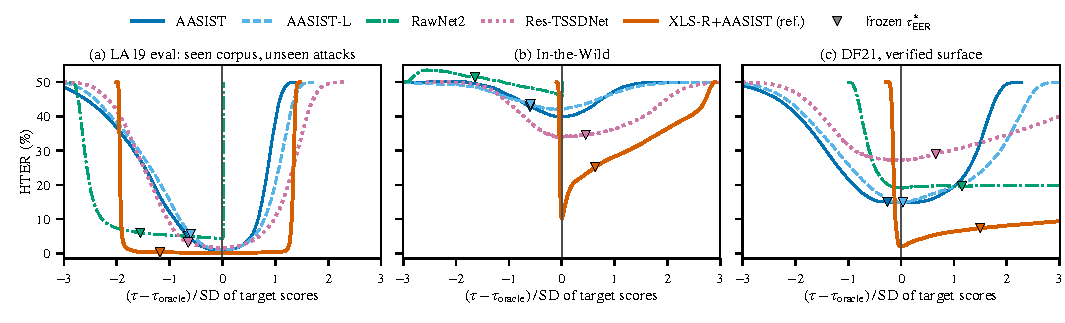
\includegraphics[width=\textwidth]{figS_sensitivity.pdf}
\caption{Threshold sensitivity. HTER against the threshold, in standard deviations of the target scores
from the target-oracle threshold (vertical line). Triangles mark the frozen \(\tauE\), and the vertical distance from a triangle to its curve's
minimum is the TTG. The near-vertical RawNet2 segment in (a) is its score ceiling at 0 (see text).}
\label{fig:sens}
\end{figure}

% src: revision/paper/supplement.tex; revision/results/
\begin{table}[!ht]
\caption{Band and miss at \(\tauE\): in SD units of the target scores (not comparable across score parametrisations) and in rank terms
(share of target clips, comparable).}
\label{tab:band}
\centering
\footnotesize
\begin{tabular}{@{}llrrrr@{}}
\toprule
Target & Model & Band (SD) & Band (\% of clips) & Miss (SD) & Miss (\% of clips) \\
\midrule
LA19 eval & AASIST & 0.68 & 3.0 & $-$0.65 & 8.2 \\
LA19 eval & AASIST-L & 0.62 & 3.3 & $-$0.60 & 9.2 \\
LA19 eval & RawNet2 & 1.02 & 6.5 & $-$1.56 & 5.0 \\
LA19 eval & Res-TSSDNet & 0.92 & 4.0 & $-$0.65 & 4.0 \\
LA19 eval & XLS-R (ref.) & 2.99 & 2.2 & $-$1.18 & 0.3 \\
\midrule
In-the-Wild & AASIST & 0.62 & 21.1 & $-$0.60 & 21.4 \\
In-the-Wild & AASIST-L & 0.82 & 25.1 & $-$0.59 & 19.7 \\
In-the-Wild & RawNet2 & 0.23 & 27.0 & $-$1.64 & 42.3 \\
In-the-Wild & Res-TSSDNet & 0.89 & 34.7 & 0.45 & 18.3 \\
In-the-Wild & XLS-R (ref.) & 0.03 & 10.0 & 0.63 & 26.8 \\
\midrule
DF21 & AASIST & 1.12 & 18.2 & $-$0.26 & 4.5 \\
DF21 & AASIST-L & 0.56 & 12.3 & 0.03 & 0.7 \\
DF21 & RawNet2 & 3.57 & 19.5 & 1.15 & 8.3 \\
DF21 & Res-TSSDNet & 1.04 & 23.0 & 0.66 & 7.3 \\
DF21 & XLS-R (ref.) & 0.20 & 4.3 & 1.50 & 1.9 \\
\bottomrule
\end{tabular}

\end{table}

% src: revision/paper/supplement.tex; revision/results/
\section{All policies on every target}
Table~\ref{tab:pol} reports FRR/FAR and TTG at the five policies on every target, with the oracle HTER (discrimination) and the
target-oracle FRR at FAR \(\le\) 5\% (the smallest target threshold whose target FAR is at most 5\%, a BPCER20-style quantity that separates
discrimination from transfer in the lenient policies). Table~\ref{tab:ttg} adds the speaker-cluster intervals of TTG at every policy. The registered clip-level interval exists for \(\tauE\) only.

% src: revision/paper/supplement.tex; revision/results/
% src: revision/paper/supplement.tex; revision/results/
\begin{table}[!ht]
\caption{FRR/FAR (\%) and TTG (pp) at the five frozen policies, the oracle HTER (\%), and the FRR (\%) at the smallest target threshold with target FAR
\(\le 5\)\%.}
\label{tab:pol}
\centering
\wide{s_tab_policies}
\end{table}

% src: revision/paper/supplement.tex; revision/results/
% src: revision/paper/supplement.tex; revision/results/
\begin{table}[!ht]
\caption{TTG (pp) with the speaker-cluster 95\% interval (\(B=1000\), seed 0) at every policy, and the registered clip-level interval at \(\tauE\).}
\label{tab:ttg}
\centering
\wide{s_tab_ttg_spk}
\end{table}

% src: revision/paper/supplement.tex; revision/results/
\section{H2 and the speaker structure of ITW}
ITW's metadata carry 54 distinct speaker labels (the dataset paper reports 58 public figures), with 14 to 3,636 clips per label (median 212.5), and the five largest labels supply 50.5\% of all clips. Every label has both classes. Table~\ref{tab:h2} repeats the H2 statistic with its
sensitivity to single speakers: deleting one speaker moves AASIST's FRR\(-\)FAR between \(-0.5\) and \(+5.4\)\,pp, and the speaker-macro average (each speaker weighted equally) differs from the pooled one. With four tests per family, Holm compares the ordered \(p\) values with 0.0125, 0.0167, 0.025 and 0.05. Table~\ref{tab:spk} summarises the per-speaker FRR at \(\tauE\)
(the analysis files use the dataset's public speaker labels, and the paper reports no speaker names). The five largest speakers supply 58\% of
the genuine clips and 51--59\% of the rejections, in proportion to their clips, so the pooled FRR is a clip-weighted average dominated by a
few heavy speakers. The metadata carry no recording identifier or condition fields, so a worst-speaker list by recording condition and a
two-way speaker-by-recording bootstrap are not possible. If recordings are nested in speakers, the speaker-level unit already absorbs
that correlation.

% src: revision/paper/supplement.tex; revision/results/
% src: revision/paper/supplement.tex; revision/results/
\begin{table}[!ht]
\caption{H2 at \(\tauE\) on ITW: pooled and speaker-macro \(\frr-\far\), the range when one speaker is deleted, the share of cluster
replicates with a positive difference, and one-sided \(p\) values (clip bootstrap \(B=1000\), speaker bootstrap \(B=10{,}000\)).}
\label{tab:h2}
\centering
\footnotesize
\setlength{\tabcolsep}{3pt}
\resizebox{\textwidth}{!}{\begin{tabular}{@{}lrrrrrr@{}}
\toprule
Model & Pooled $\frr-\far$ (pp) & Speaker-macro (pp) & Delete-one-speaker range (pp) & Cluster replicates $>0$ (\%) & $p$ (clips) & $p$ (speakers) \\
\midrule
AASIST & $+$1.86 & $+$3.34 & $-$0.5 to $+$5.4 & 63.3 & $\leq$.001 & 0.3671 \\
AASIST-L & $+$14.11 & $+$15.94 & $+$10.4 to $+$22.6 & 93.9 & $\leq$.001 & 0.0615 \\
RawNet2 & $-$35.31 & $-$27.09 & $-$43.1 to $-$30.4 & 0.3 & 1.000 & 0.9969 \\
Res-TSSDNet & $+$31.32 & $+$41.91 & $+$27.6 to $+$38.0 & 100.0 & $\leq$.001 & 0.0001 \\
\bottomrule
\end{tabular}
}
\end{table}

% src: revision/paper/supplement.tex; revision/results/
\begin{table}[!ht]
\caption{Per-speaker view of ITW at \(\tauE\) (descriptive).}
\label{tab:spk}
\centering
\wide{s_tab_speakers}
\end{table}

% src: revision/paper/supplement.tex; revision/results/
% src: revision/paper/supplement.tex; revision/results/
\begin{figure}[!ht]
\centering
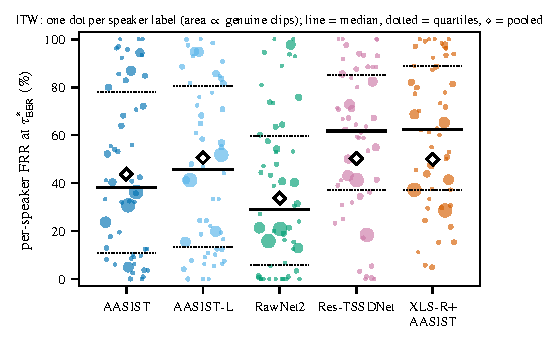
\includegraphics[width=0.62\textwidth]{figS_speakers.pdf}
\caption{ITW: FRR at \(\tauE\) per speaker label (one dot per label, area proportional to genuine clips, line = median, dotted = quartiles,
diamond = pooled FRR).}
\label{fig:spk}
\end{figure}

% src: revision/paper/supplement.tex; revision/results/
A rejection concentrated on a few speakers is more than a statistical nuisance. ITW's genuine speakers are public figures, and a detector that
rejects a speaker's authentic recordings gives anyone who wishes to deny them a tool's verdict as cover, the ``liar's dividend''
\citep{chesney19_deepfakes}. The lesson for a deployer is to estimate FRR over many speakers (Sec.~\ref{sec:cheap}).

% src: revision/paper/supplement.tex; revision/results/
\section{H5 in detail}
The 1,000-clip manifest is a uniform seeded draw within class (500 bona fide and 500 spoof, seed 20260725) from the LA19 evaluation set, frozen
before any H5 stressed audio was generated; the hypothesis predates the manifest, and DEV-2 fixes the test details.
It covers all 67 evaluation speakers (3 to 29 clips each, median 14) and all 13 attacks (28 to 53
spoofs each: A07 34, A08 32, A09 36, A10 41, A11 40, A12 47, A13 29, A14 28, A15 40, A16 34, A17 40, A18 46, A19 53). Table~\ref{tab:h5}
gives the two components of the H5 statistic with speaker-cluster intervals. \(\Delta\frr>0\) and \(\Delta\far<0\) are both significant for
all four models under Holm within each component's family. The convention for the label of the resynthesised bona fide clips, and its
competing alternatives \citep{wang23_vocoded,wu24_codecfake,xiao26_resynth}, are discussed in the paper. Under the competing convention,
the \(\Delta\frr\) column would read as detections of resynthesised speech rather than as rejections of genuine speech. We did not run a second analysis under that convention.

% src: revision/paper/supplement.tex; revision/results/
% src: revision/paper/supplement.tex; revision/results/
\begin{table}[!ht]
\caption{H5 components at \(\tauE\) (\(B=10{,}000\) speaker-cluster bootstrap, one-sided \(p\)).}
\label{tab:h5}
\centering
\wide{s_tab_h5}
\end{table}

% src: revision/paper/supplement.tex; revision/results/
% src: revision/paper/supplement.tex; revision/results/
\begin{figure}[!ht]
\centering
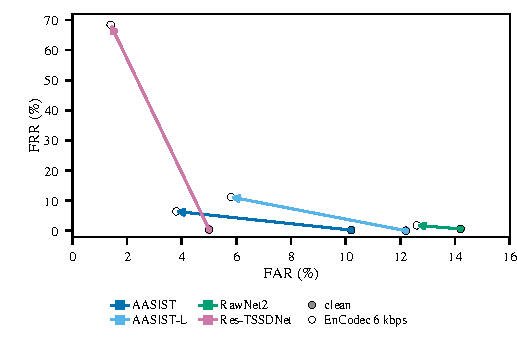
\includegraphics[width=0.62\textwidth]{figS_h5.pdf}
\caption{H5: each arrow runs from the clean copy (filled) to its EnCodec 6\,kbps resynthesis (open) at the frozen \(\tauE\) on the 1,000-clip
manifest. FRR rises and FAR falls for every model, and RawNet2's arrow is short.}
\label{fig:h5}
\end{figure}

% src: revision/paper/supplement.tex; revision/results/
\section{The silence cue}
\label{sec:silence}
\emph{Method.} Leading and trailing silence are measured after the harness's loader (16\,kHz) with an energy VAD: 25\,ms frames, 10\,ms hop,
only full frames, \(E=10\log_{10}(\overline{x^2}+10^{-12})\)\,dB, and a frame is active if within \(T\) dB of the clip's loudest frame
(\(T\in\{25,35,45\}\), with \(T=35\) as the primary). Leading silence is the start of the first active frame, and trailing silence the samples after the last. For the trimmed arm, both ends are cut at \(T=35\) with zero margin, and a clip that would fall under 0.25\,s is left untrimmed
(3 ITW clips, none in LA19). Trimming is applied at test time only: the models are not retrained. All five models were re-scored in fp32
on trimmed LA19 dev, LA19 eval and ITW. Before any trimmed run, a no-trim run on the first 200 clips of each set matched the committed scores
(\(|d|\le10^{-4}\), where the Res-TSSDNet LA19-eval gate used the platform-matched reference, Table~\ref{tab:dev}).

% src: revision/paper/supplement.tex; revision/results/
% src: revision/paper/supplement.tex; revision/results/
\begin{table}[!ht]
\caption{Leading and trailing silence by set and class (energy VAD, \(T=35\)\,dB unless stated), and leading silence alone as a bona fide
detector.}
\label{tab:sil}
\centering
\wide{s_tab_silence}
\end{table}

% src: revision/paper/supplement.tex; revision/results/
% src: revision/paper/supplement.tex; revision/results/
\begin{figure}[!ht]
\centering
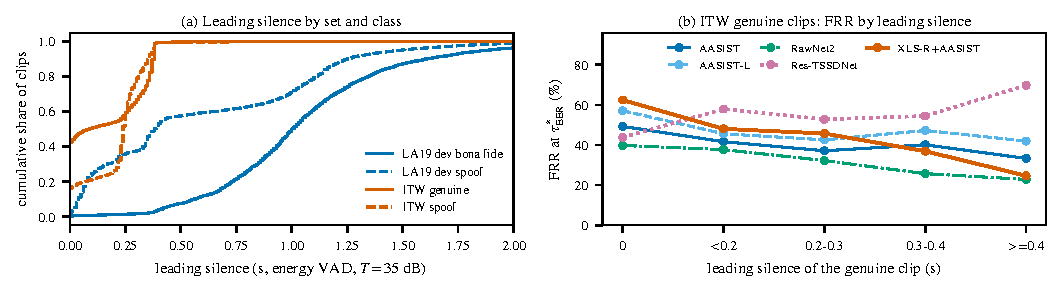
\includegraphics[width=\textwidth]{figS_silence.pdf}
\caption{(a) Cumulative distribution of leading silence. LA19 bona fide clips start with about a second of silence, ITW genuine clips with almost none, and none longer than about 0.4\,s. (b) ITW genuine clips: FRR at \(\tauE\) by leading silence.}
\label{fig:sil}
\end{figure}

% src: revision/paper/supplement.tex; revision/results/
\begin{table}[!ht]
\caption{FRR (genuine clips) and FAR (spoofs) at \(\tauE\) by leading silence, and the Spearman correlation of score and leading silence
(bona fide clips). Leading silence also tracks recording source; the correlations are descriptive, and the test-time
trimming intervention does not by itself isolate a learned silence shortcut.}
\label{tab:silfrr}
\centering
\wide{s_tab_silence_frr}
\end{table}

% src: revision/paper/supplement.tex; revision/results/
\emph{Outcome of the trimming arm.} Table~\ref{tab:trimdev} gives the dev EER and thresholds before and after trimming, and
Table~\ref{tab:trim} the target results: at the registered (untrimmed-dev) threshold on trimmed audio, at a threshold re-set on trimmed dev
scores, and the EER and oracle HTER before and after. Trimming raises the LA19 evaluation EER of all five models,
showing sensitivity to the removed non-speech. The pre-declared reading rule said that, if the ITW false-rejection pattern were mainly a silence artefact, trimming both dev and target
should shrink ITW FRR at the re-set threshold relative to the untrimmed baseline, that FRR remaining above FAR at a similar size would mean the
artefact does not explain it, and that mixed outcomes are reported as mixed. FRR does shrink for all five models, but FAR rises. The FRR-above-FAR pattern disappears for three of the four models that showed it (AASIST, Res-TSSDNet and the reference) and persists, barely
(41.5\% against 39.3\%), for AASIST-L. ITW EER moves by only \(-4.0\) to \(+3.1\)\,pp (43.0 to 46.2 for AASIST, 44.5
to 40.4 for AASIST-L, 49.0 to 49.2 for RawNet2, 34.2 to 32.9 for Res-TSSDNet and 10.5 to 13.3 for the reference),
without a consistent discrimination gain across models. Lower FRR at a more lenient threshold would also follow from
any harder development set, which this contrast cannot separate from the silence cue. We therefore report the outcome
as mixed. For the reference, dev EER rises from 0.009\% before trimming to 1.49\% after it. This documents sensitivity
of source separability and the operating point to non-speech removal, without identifying its training-time cause.

% src: revision/paper/supplement.tex; revision/results/
\emph{Comparison with earlier silence work.} \citet{muller21_silence} report that a classifier using only leading-silence duration reaches 15.1\% EER
on LA19 evaluation (ours: 17.5\% with a simple VAD at \(T=35\), 18.4\% at \(T=25\)) and that trimming silence before training raised EER from
3.6\% to 15.5\% for an established model in their experiment. Their intervention retrains on trimmed audio, ours does not, so the numbers are not comparable, but the direction (EER rises when the cue is removed) agrees.

% src: revision/paper/supplement.tex; revision/results/
\begin{table}[!ht]
\caption{Dev EER and thresholds before and after trimming (the trimmed thresholds are computed from trimmed dev scores only).}
\label{tab:trimdev}
\centering
\footnotesize
\begin{tabular}{@{}lrrrr@{}}
\toprule
Model & Dev EER (\%) & $\tauE$ & $\tauF{1}$ & $\tauA{1}$ \\
\midrule
AASIST & 0.510$\to$6.710 & $-$1.09$\to$$-$3.74 & $-$0.17$\to$$-$4.97 & $-$1.81$\to$$-$2.71 \\
AASIST-L & 0.510$\to$8.516 & $-$0.94$\to$$-$2.80 & 0.01$\to$$-$4.63 & $-$1.61$\to$$-$1.49 \\
RawNet2 & 0.549$\to$16.444 & $-$7.07$\to$$-$11.80 & $-$5.18$\to$$-$12.35 & $-$8.26$\to$$-$9.90 \\
Res-TSSDNet & 0.722$\to$10.482 & $-$8.24$\to$$-$13.30 & $-$7.05$\to$$-$16.41 & $-$9.22$\to$$-$3.78 \\
XLS-R (ref.) & 0.009$\to$1.491 & $-$1.75$\to$$-$3.57 & 3.58$\to$$-$3.59 & $-$3.53$\to$$-$3.56 \\
\bottomrule
\end{tabular}

\end{table}

% src: revision/paper/supplement.tex; revision/results/
% src: revision/paper/supplement.tex; revision/results/
\begin{table}[!ht]
\caption{Trimming both ends of every clip (\(T=35\)\,dB), LA19 evaluation and ITW. Columns three to five: FRR/FAR (\%) with (HTER \%, TTG pp) at
the registered threshold on untrimmed audio, at the same threshold on trimmed audio, and at the threshold re-set on trimmed dev scores (trimmed
audio).}
\label{tab:trim}
\centering
\wide{s_tab_trim}
\end{table}

% src: revision/paper/supplement.tex; revision/results/
\section{A check from genuine channel speech}
\label{sec:cheap}
On ITW, for each of 1,000 random splits of the 54 speaker labels into a calibration half (27) and a held-out half (27), \(k\in\{50,100,500\}\)
genuine clips were drawn uniformly from the calibration half. (i) The FRR at the shipped \(\tauE\) was estimated from the sample and compared
with the genuine FRR of the held-out speakers. (ii) \(\tau_{\mathrm{new}}\) was set at the \((\lfloor 0.01k\rfloor+1)\)-th smallest sample
score (the largest threshold whose sample FRR is at most 1\%, using no attack data), and the held-out FRR and FAR (spoofs of held-out speakers) were
measured at it. Table~\ref{tab:cheap} gives medians and 5--95\% ranges (seed 0). The median estimation error is near zero, but the spread across
speaker splits is about \(\pm18\)--26\,pp and does not shrink with \(k\): the limit is the number of speakers (the top five of ITW's 54
labels supply 51--59\% of the rejections), not the number of clips. Re-setting restores the FRR budget and pays for it in FAR, as expected
for a model that does not discriminate on the channel (AUC on ITW: AASIST 0.60, AASIST-L 0.59, RawNet2 0.51, Res-TSSDNet 0.73, reference 0.96).
Collecting consented genuine speech raises privacy questions that a deployer must settle first.

% src: revision/paper/supplement.tex; revision/results/
% src: revision/paper/supplement.tex; revision/results/
\begin{table}[!ht]
\caption{Genuine-speech check on ITW (1,000 speaker-disjoint splits). Estimate error = FRR estimated from the \(k\) calibration clips at the
shipped threshold minus the held-out FRR at it.}
\label{tab:cheap}
\centering
\wide{s_tab_cheap}
\end{table}

% src: revision/paper/supplement.tex; revision/results/
\section{Cost sweep, break-even and stability}
Fig.~\ref{fig:cost} plots the normalised cost \(C(p)\) of the main paper's cost definition over the effective bona fide prior \(p\) (a cost curve in the sense
of \citealp{drummond06_costcurves}, and the application-independent view of \citealp{brummer06_calibration}) at \(\tauE\), with the target-oracle cost dotted and the two registered points marked. A detector helps where \(C<1\). Table~\ref{tab:cost} gives the window of priors for each policy, and the cost of the oracle threshold at the two registered points. For
the screening model \(C=19\,\frr+\far\), so \(C<1\) requires \(\frr<(1-\far)/19\). At \(\tauE\) on ITW this is 3.1, 3.3, 1.6, 4.3 and 5.2\% for
AASIST, AASIST-L, RawNet2, Res-TSSDNet and the reference, against FRR of 43.8, 50.6, 33.8, 50.3 and 49.9\% obtained. Table~\ref{tab:stab}
gives, per target, policy and measure, the model with the largest gap in the point estimate and the share of 1,000 paired speaker-bootstrap replicates in which it is the largest. Table~\ref{tab:costsplit} splits the registered costs at \(\tauE\) into the cost of the target-oracle threshold (discrimination) and the remainder (transfer). On ITW under screening the oracle costs 0.86--1.00 and the remainder, 6.10--8.99, is transfer: the transferred threshold sits far from the accept-almost-everything point that a 0.95 prior favours, although even the best threshold barely beats the trivial system. The share of the excess that is transfer therefore depends on the cost model; at equal costs it is 2--11\% for the primary models on ITW. Under the forensic model the reference's transfer part on ITW is 0.07.

% src: revision/paper/supplement.tex; revision/results/
\begin{figure}[!ht]
\centering
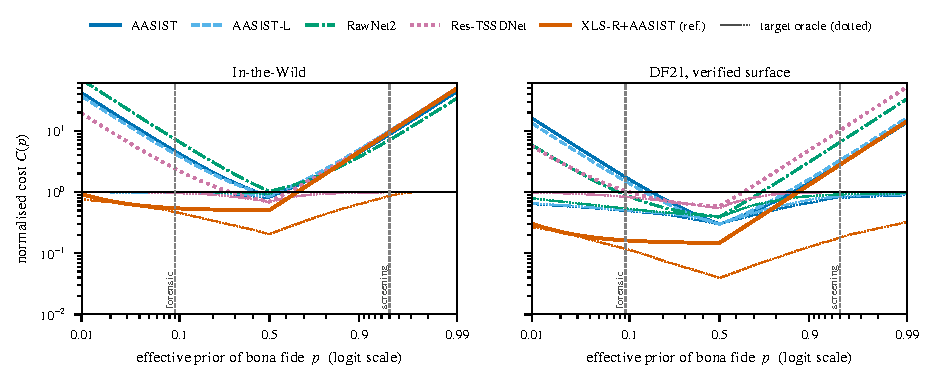
\includegraphics[width=\textwidth]{figS_cost.pdf}
\caption{Normalised cost against the effective prior of bona fide, at \(\tauE\) (solid) and at the target-oracle threshold (dotted), with the two registered points marked.}
\label{fig:cost}
\end{figure}

% src: revision/paper/supplement.tex; revision/results/
% src: revision/paper/supplement.tex; revision/results/
\begin{table}[!ht]
\caption{Break-even windows (the priors \(p\) at which \(C<1\)) and the cost of the target-oracle threshold at the screening (\(p=0.95\)) and
forensic (\(p=1/11\)) points. The last column is the largest prior at which the oracle still gains 10\% over the better trivial system.}
\label{tab:cost}
\centering
\wide{s_tab_cost}
\end{table}

% src: revision/paper/supplement.tex; revision/results/
\begin{table}[!ht]
\caption{The registered cost check at \(\tauE\): normalised cost at the transferred threshold, the cost of the target-oracle threshold (discrimination) and the remainder (transfer).}
\label{tab:costsplit}
\centering
\footnotesize
\begin{tabular}{@{}lrrrrrr@{}}
\toprule
 & \multicolumn{3}{c}{Screening ($p=0.95$)} & \multicolumn{3}{c}{Forensic ($p=1/11$)} \\
\cmidrule(lr){2-4}\cmidrule(lr){5-7}
Model & $C(\tauE)$ & oracle & transfer & $C(\tauE)$ & oracle & transfer \\
\midrule
\multicolumn{7}{@{}l}{\emph{In-the-Wild}} \\
AASIST & 8.73 & 1.00 & 7.73 & 4.63 & 0.98 & 3.65 \\
AASIST-L & 9.99 & 1.00 & 8.99 & 4.16 & 0.98 & 3.18 \\
RawNet2 & 7.10 & 1.00 & 6.10 & 7.24 & 0.99 & 6.25 \\
Res-TSSDNet & 9.74 & 0.99 & 8.75 & 2.40 & 0.97 & 1.43 \\
XLS-R (ref.) & 9.49 & 0.86 & 8.62 & 0.54 & 0.47 & 0.07 \\
\midrule
\multicolumn{7}{@{}l}{\emph{DF21, verified subset}} \\
AASIST & 2.79 & 0.81 & 1.98 & 1.76 & 0.49 & 1.27 \\
AASIST-L & 3.26 & 0.83 & 2.43 & 1.49 & 0.51 & 0.99 \\
RawNet2 & 6.45 & 0.92 & 5.54 & 0.90 & 0.53 & 0.36 \\
Res-TSSDNet & 10.09 & 1.00 & 9.09 & 1.05 & 0.84 & 0.21 \\
XLS-R (ref.) & 2.77 & 0.18 & 2.59 & 0.16 & 0.12 & 0.04 \\
\midrule
\multicolumn{7}{@{}l}{\emph{LA19 eval: seen corpus, unseen attacks}} \\
AASIST & 0.13 & 0.09 & 0.04 & 0.98 & 0.05 & 0.93 \\
AASIST-L & 0.13 & 0.09 & 0.04 & 1.11 & 0.07 & 1.05 \\
RawNet2 & 0.21 & 0.21 & 0.00 & 1.15 & 0.31 & 0.84 \\
Res-TSSDNet & 0.11 & 0.10 & 0.01 & 0.61 & 0.12 & 0.49 \\
XLS-R (ref.) & 0.02 & 0.01 & 0.00 & 0.05 & 0.01 & 0.04 \\
\bottomrule
\end{tabular}

\end{table}

% src: revision/paper/supplement.tex; revision/results/
% src: revision/paper/supplement.tex; revision/results/
\begin{table}[!ht]
\caption{Stability of the model with the largest gap, over 1,000 paired speaker-bootstrap replicates.}
\label{tab:stab}
\centering
\footnotesize
\begin{tabular}{@{}llll@{}}
\toprule
Policy & Largest HTER gap & Largest screening-cost gap & Largest forensic-cost gap \\
\midrule
\multicolumn{4}{@{}l}{\emph{LA19 eval: seen corpus, unseen attacks}} \\
$\tauE$ & AASIST-L (97.3\%) & AASIST-L (57.5\%) & AASIST-L (99.9\%) \\
$\tauF{1}$ & AASIST-L (96.5\%) & XLS-R (100.0\%) & RawNet2 (100.0\%) \\
$\tauF{5}$ & XLS-R (100.0\%) & XLS-R (98.6\%) & RawNet2 (100.0\%) \\
\midrule
\multicolumn{4}{@{}l}{\emph{In-the-Wild}} \\
$\tauE$ & XLS-R (100.0\%) & AASIST-L (47.8\%) & RawNet2 (100.0\%) \\
$\tauF{1}$ & XLS-R (100.0\%) & XLS-R (100.0\%) & RawNet2 (100.0\%) \\
$\tauF{5}$ & XLS-R (100.0\%) & AASIST (81.3\%) & RawNet2 (92.1\%) \\
\midrule
\multicolumn{4}{@{}l}{\emph{DF21, verified subset}} \\
$\tauE$ & XLS-R (99.5\%) & Res-TSSDNet (100.0\%) & AASIST (100.0\%) \\
$\tauF{1}$ & XLS-R (100.0\%) & Res-TSSDNet (100.0\%) & AASIST (100.0\%) \\
$\tauF{5}$ & XLS-R (100.0\%) & Res-TSSDNet (100.0\%) & XLS-R (100.0\%) \\
\bottomrule
\end{tabular}

\end{table}

% src: revision/paper/supplement.tex; revision/results/
\emph{Hard decisions and triage.} The cost model assumes a hard decision. Where scores only prioritise human review or allow the system to abstain
(selective classification \citep{geifman17_selective}), ranking matters and a transferred threshold bites through the review budget. The last
column of Table~\ref{tab:interval} shows the size of that effect for a three-zone policy whose review band is the interval of thresholds that
tie on dev: 47.8\% of ITW genuine clips for the reference, 12.1\% and 10.6\% for AASIST and AASIST-L. This round-1 illustration did not optimise a three-zone policy; the registered extension evaluates the separate review-budget policies described in the main text.

% src: revision/paper/supplement.tex; revision/results/
\section{DF21 documentation}
The 533,928 evaluation trials of DF21 come from the public Zenodo release (DOI 10.5281/zenodo.4835108, four parts, checksums verified). The
current reference decoder, libFLAC 1.4.3 (libsndfile 1.2.2, through soundfile 0.14.0, wraps it), rejects 228,403 of them (42.8\%) across both
labels and all nine conditions. The files were written by libFLAC 1.3.2, and their STREAMINFO and first-frame headers are identical for failing
and clean files (blocksize 4096, 16\,kHz, mono, 16-bit). The 2021-era decoder libFLAC 1.3.4 decodes all of them (ffmpeg 7.0.2 gave identical
output on a 150-file check). Of these, 149,983 pass the file's own STREAMINFO MD5 (class A, true audio) and 78,420 fail it (class B), so their
decodable audio is not what the encoder was given. On the failing files no available decode (ffmpeg, libFLAC 1.3.4, libFLAC 1.4.3 with errors tolerated) reproduces the
organisers' scores (median \(|d|\) 0.6--1.2, under 5\% of trials within \(10^{-3}\)), so the audio scored in 2021 cannot be recovered from the
public files. We score the \emph{verified subset} (evaluation minus class B: 455,508 trials, decoded by libFLAC 1.3.4 with the MD5 checked at
load) and use the 305,525 trials that decode without issue as a sensitivity subset.

% src: revision/paper/supplement.tex; revision/results/
Table~\ref{tab:df21} breaks the evaluation set down by condition and integrity class. The exclusions are not uniform: they remove 18.8\% of bona
fide trials and 14.6\% of spoof trials, and the class-B share differs by source corpus (asvspoof 15.0\%, vcc2018 9.6\%, vcc2020 18.2\%
of that source's evaluation trials, that is 12,257, 17,787 and 48,376 trials) and mildly by condition (13.1--16.8\%). The key file also lists the
\texttt{hidden} (18,576 trials, all of type \texttt{trim}) and \texttt{progress} (59,325 trials) subsets of ASVspoof~2021. They are not part of any
registered surface, their FLAC integrity is unclassified, and we did not score them, so the question whether the hidden subsets (from which
non-speech intervals were removed) behave differently remains open. Published DF21 figures are not comparable with ours.

% src: revision/paper/supplement.tex; revision/results/
% src: revision/paper/supplement.tex; revision/results/
\begin{table}[!ht]
\caption{DF21 evaluation trials by media condition and FLAC integrity class: class A (libFLAC 1.4 rejects the file, 1.3 decodes it and the MD5
verifies), class B (MD5 fails), the verified subset (evaluation minus B) and the clean subset (evaluation minus A and B).}
\label{tab:df21}
\centering
\wide{s_tab_df21}
\end{table}

\section{Round 2: registration events and additional results}
\label{sec:r2supp}
% src: DEVIATIONS.md DEV-9; PREREGISTRATION_ROUND2.md
\subsection{Registration events}
Round~2 has its own registration, frozen in version control at the tag \texttt{round2-freeze} on 7~October 2026 with
its analysis code, and five amendments (Table~\ref{tab:dev2}). Each amendment was written into the deviation log before
the work it governs and records what had been seen when it was written. None changes a registered test, support rule or
threshold.

% src: DEVIATIONS.md DEV-9; DEVIATIONS.md DEV-9 amendment 1; DEVIATIONS.md DEV-9 amendment 2; DEVIATIONS.md DEV-9 amendment 3; DEVIATIONS.md DEV-9 amendment 4; DEVIATIONS.md DEV-9 amendment 5
\begin{table}[!ht]
\caption{Round-2 registration events.}
\label{tab:dev2}
\centering
\footnotesize
\setlength{\tabcolsep}{3pt}
\begin{tabular}{@{}p{0.13\textwidth}p{0.08\textwidth}p{0.40\textwidth}p{0.33\textwidth}@{}}
\toprule
Event & Date & What it fixed or changed & What had been seen \\
\midrule
Registration & 7 Oct 2026 & Three detectors, eleven AASIST-L runs, eight channel conditions, gates, thresholds, R2-H1 to R2-H4,
the reading rule, exploratory analyses and failure rules. & Every round-1 result and published figures; pre-tag smoke
tests on LA19 training clips only. No round-2 score and no audio of the new channel conditions. \\
Amendment 1 & 7 Oct 2026 & A run that fails from resource exhaustion before completing its first epoch is relaunched
once; runs start only when their GPU has room. & The out-of-memory failures; no development score or training metric. \\
Amendment 2 & 7 Oct 2026 & E9 uses the exact unpenalised logistic fit instead of a fixed-step routine that underfits.
& A unit test on synthetic scores; no E9 quantity. \\
Amendment 3 & 7 Oct 2026 & FLAC audio is accepted only if it matches its STREAMINFO MD5 and is converted to float by
the harness; XLSR-Mamba's DF21 scores are re-scored. & Decoder comparisons; the affected score file existed, but no
quantity had been computed from it. \\
Amendment 4 & 8 Oct 2026 & One unchanged rerun of Pascu's MLAAD-5 scoring on a GPU without a training run. & The
out-of-memory log and the clip durations; no score. \\
Amendment 5 & 10 Oct 2026 & For Pascu's detector, a clip shorter than 400 samples is repeated to 400 samples and logged;
one more rerun. & The failure log and the shortest clip lengths; no score. \\
\bottomrule
\end{tabular}
\end{table}

% src: results/round2/gates.json; results/round2/pascu/head_train.json; DEVIATIONS.md DEV-9 amendment 1; DEVIATIONS.md DEV-9 amendment 5
\subsection{Execution}
All eleven AASIST-L runs trained for 100 epochs without divergence or NaN loss; amendment~1 covered a launch that ran out
of GPU memory before any epoch finished. The weight averages of the untrimmed runs hold 1 to 12 snapshots. No trimmed run
reached the averaging threshold, so each trimmed model is its last epoch and scores identically to its last-epoch copy.
The head of Pascu's detector was fitted on the 25,380 LA19 training clips (L-BFGS, 100 iterations, no convergence
warning, training accuracy 1.0). Pascu's MLAAD-5 scoring failed twice, first for lack of GPU memory and then on two
186-sample clips; the amendment-5 rerun scored all 494,853 trials and repeated exactly those two clips. XLSR-Mamba's DF21
scores were recomputed under amendment~3, and the quarantined file entered no analysis.

% src: gen/r2s_policies.tex; results/round2/analysis/r2_explore.json (E1_E8_E10)
\subsection{All policies, BPCER at fixed APCER and break-even windows}
Table~\ref{tab:r2pol} gives the round-2 detectors at all five policies (E1), BPCER at the development thresholds for
APCER budgets of 1\% and 5\% against the target threshold that achieves those APCERs (E8), and the bona fide priors at
which the cost at \(\tauE\) is below 1 (E10). The FAR budgets do not keep their APCER after transfer: on ITW, \(\tauA{1}\)
gives an APCER of 8.4\% for Pascu's detector and 10.9\% for XLSR-Mamba. Pascu's detector has no break-even window on
MLAAD-5.

% src: gen/r2s_policies.tex; results/round2/analysis/r2_explore.json (E1_E8_E10)
\begin{table}[!ht]
\caption{Round-2 detectors: FRR/FAR (\%) at the five frozen policies, BPCER@\(k\) = BPCER at the dev threshold for
APCER \(k\)\% / at the target threshold with APCER \(k\)\%, and the break-even window of bona fide priors at \(\tauE\).}
\label{tab:r2pol}
\centering
\wide{r2s_policies}
\end{table}

% src: gen/r2s_last.tex; results/round2/analysis/r2_explore.json (E2_E3)
\subsection{Weight averaging and last-epoch weights}
Table~\ref{tab:r2last} sets the registered untrimmed models (weight averages) beside their last-epoch weights and the
trimmed models (E3). Averaging lowers the transfer gap on both targets (LA19 eval mean 2.69 against 7.59\,pp, ITW 6.51
against 10.49\,pp) at similar EER. With last-epoch weights in both arms, trimming lowers mean ITW FRR from 23.4\% to 16.8\%
and raises mean ITW FAR from 71.6\% to 86.5\%, and mean ITW EER rises from 40.7\% to 43.8\%. These are exploratory
comparisons of five runs per arm, without a test.

% src: gen/r2s_last.tex; results/round2/analysis/r2_explore.json (E2_E3)
\begin{table}[!ht]
\caption{Untrimmed AASIST-L runs with their registered weight averages and with their last-epoch weights, and the trimmed
runs, at each run's \(\tauE\) (rates \%, TTG pp). \(^\dagger\)Pipeline check, outside the means.}
\label{tab:r2last}
\centering
\wide{r2s_last}
\end{table}

% src: gen/r2s_channels.tex; results/round2/analysis/r2_explore.json (E4)
\subsection{Channel effects per training run}
Table~\ref{tab:r2chanruns} gives the channel effects of every training run; the main paper prints the arm means. The
differences between arms under noise and EnCodec hold for every seed.

% src: gen/r2s_channels.tex; results/round2/analysis/r2_explore.json (E4)
\begin{table}[!ht]
\caption{Channel effects at each run's \(\tauE\): \(\Delta\)FRR/\(\Delta\)FAR (pp) against the clean copy of the 1,000-clip
set (E4).}
\label{tab:r2chanruns}
\centering
\wide{r2s_channels}
\end{table}

% src: gen/r2s_threezone.tex; gen/r2s_budgets.tex; results/round2/analysis/r2_explore.txt (E7)
\subsection{Three-zone review on every target and at other budgets}
Tables~\ref{tab:r2threeall} and~\ref{tab:r2budgets} extend the review analysis (E7). The development-designed band
exceeds its 10\% budget on every target for the LA19-trained detectors, even on LA19 eval (20.3--40.4\%), whose genuine
speech comes from the source corpus; on MLAAD-5 it reaches 52.2--96.2\%. Larger budgets move little: at 20\%, the band
of XLSR-Mamba still sends 77.7\% of ITW clips to review. For the round-1 primary models, which barely discriminate ITW,
even the target-oracle band leaves 58.1--67.3\% of genuine clips auto-rejected for AASIST, AASIST-L and RawNet2 at the
10\% budget.

% src: gen/r2s_threezone.tex; results/round2/analysis/r2_explore.json (E7)
\begin{table}[!ht]
\caption{Three-zone review at the 10\% dev budget on every target (E7; \% of target clips; columns as in the main
paper's ITW table: Gen.\ in review = genuine clips sent to review, Gen.\ rej.\ = genuine clips rejected automatically,
Spoof acc.\ = spoofs accepted automatically).}
\label{tab:r2threeall}
\centering
\wide{r2s_threezone}
\end{table}

% src: gen/r2s_budgets.tex; results/round2/analysis/r2_explore.json (E7)
\begin{table}[!ht]
\caption{Three-zone review on ITW at review budgets of 5, 10 and 20\% of dev traffic: the band designed on dev, the same
budget at the labelled target oracle, and the label-free re-anchoring (E7; \% of ITW clips; Rej. = genuine clips
auto-rejected; Acc. = spoofs auto-accepted).}
\label{tab:r2budgets}
\centering
\wide{r2s_budgets}
\end{table}

% src: gen/r2s_calibration.tex; results/round2/analysis/r2_explore.json (E9); DEVIATIONS.md DEV-9 amendment 2
\subsection{Calibrated cost at other priors}
Table~\ref{tab:r2calpri} gives actual and minimum cost after the source-dev logistic calibration at bona fide priors with
logit \(-2\) and \(+2\) (about 0.12 and 0.88) besides equal priors (E9). At logit \(-2\) the minimum cost on MLAAD-5 is 1.00
for every detector, so no threshold on these scores beats rejecting everything there; at logit \(+2\) every detector's
actual cost on ITW exceeds 1.

% src: gen/r2s_calibration.tex; results/round2/analysis/r2_explore.json (E9)
\begin{table}[!ht]
\caption{Actual/minimum normalised cost after logistic calibration on source dev, at three bona fide priors (E9).}
\label{tab:r2calpri}
\centering
\footnotesize
% generated by analysis/round2/r2_paper_tables.py from results/round2/analysis/r2_explore.json (E9); do not edit by hand
% actual/minimum normalised cost after an exact logistic calibration on source dev (DEV-9 amendment 2), prior-corrected, at logit(prior of bona fide) -2, 0, +2; 1 = the better trivial system
\begin{tabular}{@{}llrrr@{}}
\toprule
Model & Target & logit \(-2\) & logit 0 & logit \(+2\) \\
\midrule
AS5 AASIST & LA19 eval & 1.64/1.00 & 0.61/0.59 & 0.89/0.76 \\
AS5 AASIST & ITW & 1.00/0.80 & 0.75/0.54 & 1.52/0.98 \\
AS5 AASIST & DF21 ver. & 1.11/1.00 & 0.53/0.51 & 0.89/0.80 \\
AS5 AASIST & MLAAD-5 & 1.07/1.00 & 0.84/0.72 & 0.99/0.92 \\
AS5 AASIST & AS5 eval & 1.03/1.00 & 0.55/0.55 & 0.91/0.82 \\
\addlinespace
Pascu LR & LA19 eval & 0.19/0.05 & 0.04/0.01 & 0.05/0.02 \\
Pascu LR & ITW & 0.38/0.37 & 0.23/0.15 & 1.18/0.41 \\
Pascu LR & DF21 ver. & 0.18/0.16 & 0.12/0.06 & 0.60/0.15 \\
Pascu LR & MLAAD-5 & 2.26/1.00 & 1.09/0.76 & 5.80/0.90 \\
\addlinespace
XLSR-Mamba & LA19 eval & 0.05/0.01 & 0.01/0.00 & 0.02/0.01 \\
XLSR-Mamba & ITW & 0.56/0.40 & 0.44/0.18 & 2.58/0.39 \\
XLSR-Mamba & DF21 ver. & 0.10/0.09 & 0.06/0.03 & 0.28/0.07 \\
XLSR-Mamba & MLAAD-5 & 3.50/1.00 & 0.64/0.60 & 1.31/0.93 \\
\addlinespace
AASIST & LA19 eval & 0.19/0.05 & 0.08/0.02 & 0.20/0.06 \\
AASIST & ITW & 1.72/0.97 & 0.84/0.80 & 2.88/1.00 \\
AASIST & DF21 ver. & 0.90/0.47 & 0.30/0.30 & 0.81/0.63 \\
AASIST & MLAAD-5 & 2.99/1.00 & 0.64/0.52 & 1.01/0.98 \\
\addlinespace
AASIST-L & LA19 eval & 0.20/0.06 & 0.09/0.02 & 0.21/0.06 \\
AASIST-L & ITW & 1.57/0.97 & 0.86/0.84 & 3.16/1.00 \\
AASIST-L & DF21 ver. & 0.73/0.49 & 0.30/0.30 & 1.00/0.70 \\
AASIST-L & MLAAD-5 & 2.78/1.00 & 0.66/0.61 & 1.08/0.98 \\
\addlinespace
RawNet2 & LA19 eval & 0.71/0.27 & 0.11/0.08 & 0.16/0.15 \\
RawNet2 & ITW & 4.32/0.99 & 1.02/0.92 & 2.94/1.00 \\
RawNet2 & DF21 ver. & 0.64/0.51 & 0.39/0.38 & 2.50/0.84 \\
RawNet2 & MLAAD-5 & 3.80/1.00 & 0.62/0.55 & 0.89/0.85 \\
\addlinespace
Res-TSSDNet & LA19 eval & 0.19/0.10 & 0.05/0.03 & 0.14/0.07 \\
Res-TSSDNet & ITW & 1.20/0.95 & 0.70/0.68 & 2.92/0.97 \\
Res-TSSDNet & DF21 ver. & 0.82/0.80 & 0.59/0.54 & 3.50/0.98 \\
Res-TSSDNet & MLAAD-5 & 1.49/1.00 & 0.82/0.75 & 3.67/0.96 \\
\addlinespace
XLS-R+AASIST & LA19 eval & 0.03/0.01 & 0.00/0.00 & 0.01/0.01 \\
XLS-R+AASIST & ITW & 0.57/0.42 & 0.53/0.20 & 3.60/0.58 \\
XLS-R+AASIST & DF21 ver. & 0.17/0.10 & 0.16/0.04 & 1.04/0.12 \\
XLS-R+AASIST & MLAAD-5 & 2.30/1.00 & 0.50/0.49 & 1.67/0.94 \\
\bottomrule
\end{tabular}

\end{table}

% src: revision/paper/supplement.tex; revision/results/
\section{Reproducibility}
The archived round-1 inputs include: the fp32 score files of the five models on every surface, the frozen thresholds (never changed), the metadata files
(sha256 recorded), and the manifests. Each analysis script recomputes 45 model-by-target-by-policy cells, the thresholds, H2, H5, the cost and
oracle numbers from the score files and stops unless they equal the committed values to \(10^{-12}\). The figures and the tables of the
paper and of this supplement are generated from the result files by scripts.

\bibliographystyle{elsarticle-harv}
\bibliography{refs}

\end{document}
